\chapter{Referencial Teórico}

\section{Mercado imobiliário}

Todo ser humano por natureza precisa de uma habitação, sendo isso uma necessidade ligada a procura de uma maior segurança contra as várias adversidades do ambiente externo. No entanto, essa necessidade de consumo por uma habitação atualmente se divide em dois principais grupos: aquelas pessoas que realmente investem em uma moradia com a finalidade de satisfazer essa necessidade básica de maior proteção, e também, aqueles indivíduos que compram com a finalidade de aumentar seu capital financeiro ou compor a base de sua economia \cite{Arraes:2008}.

Um dos setores imobiliários que administra esses consumos é o setor terciário, que envolve as atividades do mercado imobiliário (compra, venda e locação) e será o contexto principal deste trabalho. Esse setor é de suma importância para o mercado nacional, pois é gerador de emprego, renda e altos níveis de investimentos. Uma das particularidades relevantes desse setor é a sua importante participação nas características de desenvolvimento de uma nação. Com essa importância, o governo tende a incentivar essa área, com o intuito de estimular os negócios imobiliários para que estimule o país a se desenvolver \cite{Correa:2018}.

O setor imobiliário é muito importante para a sociedade, entretanto, como todo setor econômico, é necessário com que negócios sempre estejam a frente em novidades do mercado, para que possam dar certo e expandir. Um processo muito utilizado por imobiliárias nos dias atuais é o \textit{marketing} digital que também será abordado neste trabalho.

\subsection{\textit{Marketing} Digital}

Um dos meios mais poderosos utilizado pelas imobiliárias para atrair visitantes, que talvez virem futuros clientes, é o \textit{marketing} em meio digital, que disponibiliza serviços e conteúdos de qualidade aos seus possíveis clientes. Por meio dele é possível oferecer oportunidades para uma mobiliária se relacionar com seus clientes \cite{Barreto:2019}.

Como qualquer outro processo, o \textit{marketing} digital também precisa de estudo e aperfeiçoamento constante, dado que em cada etapa há perda de pessoas (clientes). Dessa forma, a representação ilustrativa desse tipo de ocorrência é mais conhecida como funil de \textit{marketing} digital \cite{BORGES:2017}.

É fortemente recomendado que toda e qualquer empresa deve planejar seu processo, desde a atração do visitante, feita por meio da propaganda, até a aquisição do cliente que antes era simplesmente um visitante interessado em atender seus próprios objetivos. Além de planejar, também deve ocorrer o acompanhamento de toda a trajetória do visitante até conversão deste em cliente \cite{INSIDEOUT:2018}.
Segundo o \textit{site} \textit{site} Agenciainsideout.com (\citeyear{INSIDEOUT:2018}), o funil de \textit{marketing} ajuda no andamento de vendas e aquisição de clientes, gerando certos benefícios, tais como:

\begin{itemize}
    \item Melhoria na gestão;
    
    \item Previsão de resultados;
    
    \item Aumento de produtividade;
    
    \item Mais oportunidades de negócios com \textit{leads} qualificados;
    
    \item Evolução na estratégia de aquisição de \textit{leads};
    
    \item Melhoramento do produto.

\end{itemize}

\begin{figure}[H]
    \centering
    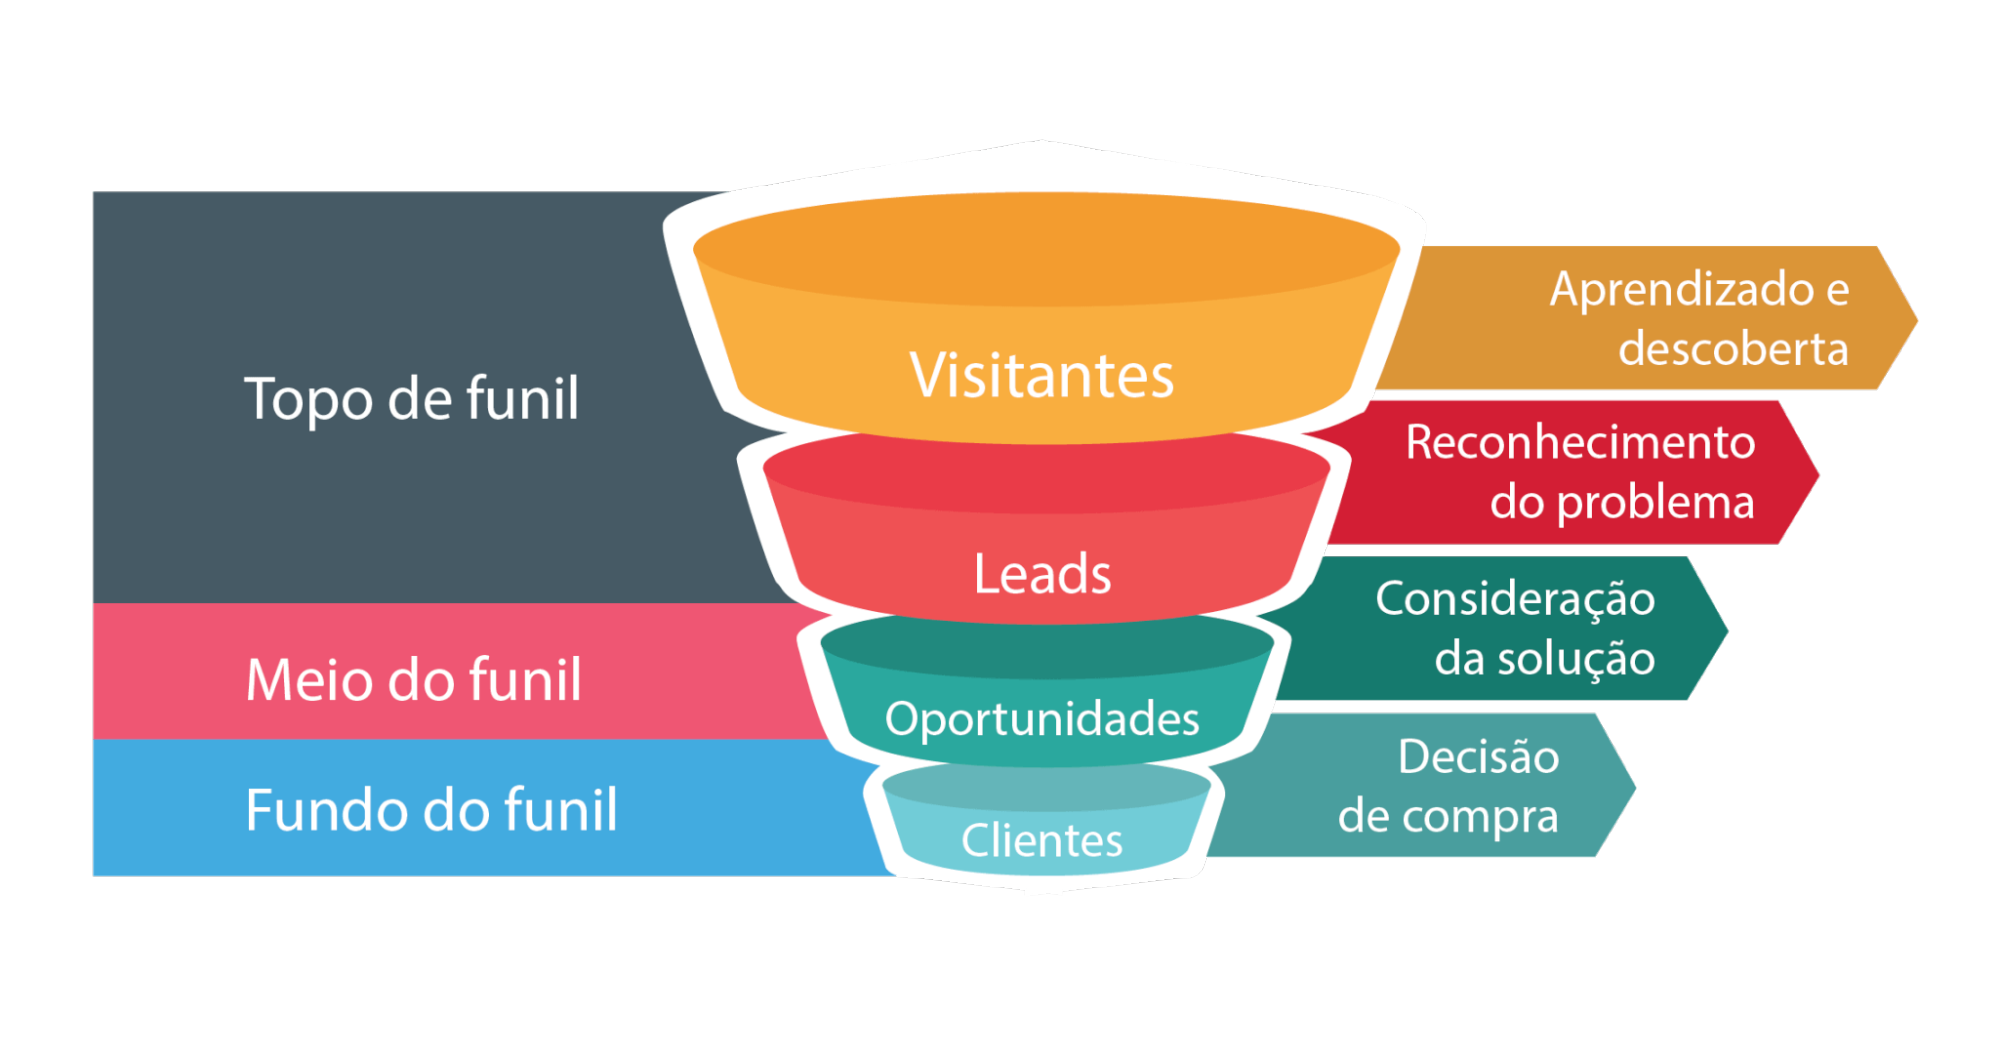
\includegraphics[scale=0.2]{figuras/referencial_teorico/funil_marketing.png}
    \caption[Funil de \textit{marketing} digital]{Funil de \textit{marketing} digital. Fonte: \cite{INSIDEOUT:2018}.}
    \label{fig:funil_marketing}
\end{figure}

Como descrito pelo site Agenciainsideout.com (\citeyear{INSIDEOUT:2018}), pode ser observado na Figura \ref{fig:funil_marketing}, que o funil tem quatro fases principais, sendo que podem ser feitas mudanças de acordo com o contexto de cada empresa. Para maior aprofundamento, há a descrição de cada uma dessas fases a seguir:

\begin{itemize}
    \item 1ª fase - Aquisição (visitante): o visitante entra no ambiente virtual da empresa por algum motivo, seja por meio de anúncios em outra página virtual disponível na Internet ou por alguma pesquisa que fez. Um fator considerado importante nesta etapa é atrair o visitante para continuar a usar o sítio virtual da empresa para atender ao seu objetivo, mesmo ainda não sendo totalmente conhecido, retornando a ele e o compartilhando com outras pessoas. Algumas características importantes que podem ajudar nisso são disponibilizar conteúdos sempre recentes e também oferecer uma usabilidade interessante;
    
    \item 2ª fase - Ativação (\textit{lead}): o visitante fornece algumas informações de contato, como por exemplo: nome completo, e-mails, telefones e entre outros, em troca de algum conteúdo, geralmente o que seria o chamado \textit{lead}. Para obter mais \textit{leads} é aconselhado verificar se há muitas perguntas ou se há alguma pergunta de teor evasivo;
    
    \item 3ª fase - Retenção (oportunidade): agora que já foi adquirida algumas informações de contato é necessário começar a se relacionar com o visitante. Um fator recomendado é ajudar o visitante para que ele fique mais interessado, como por exemplo, dar uma amostra grátis de algum serviço ou parte de tal serviço. E também, analisar, se possível, o histórico daquele usuário para compreender melhor quais poderiam ser os interesses dele;
    
    \item 4ª fase - Receita (cliente): com o relacionamento estabelecido, o visitante se torna finalmente um cliente, após esse acontecimento é muito importante medir o nível de satisfação do cliente com o produto ou serviço, ou seja, uma fidelização da parte do cliente com a empresa, e além disso, se está ocorrendo recomendação de sua empresa pelo cliente.

\end{itemize}

Como pôde ser visto, o \textit{e-commerce} é importante aliado do \textit{marketing} digital de empresas do setor imobiliário, entre outras, principalmente na 1ª fase de aquisição do visitante. Por ser de grande relevância, é importante conhecer o \textit{e-commerce} um pouco mais para o desenvolvimento consciente deste trabalho.

\subsection{\textit{E-commerce}}

O comércio eletrônico ou \textit{e-commerce}, como também é chamado, surgiu e ficou famoso na década de 90, com a ajuda da popularização da Internet e de empresas pioneiras neste setor como Ebay e Amazon.com. Esse tipo de comércio oferecia a opção de compra de qualquer produto das empresas através de seus serviços fornecidos pela rede mundial de computadores, podendo realizar a busca de um produto específico e mostrar outros que fossem relacionados àquele que estava sendo visualizado. Com os avanços de conexão e da segurança na Internet tornou-se possível que os seus usuários pagassem pelo próprio produto virtualmente e os recebesse em sua moradia, envolvendo também os serviços de postagem ou entrega comercial \cite{Nakamura:2011}.

Smith, Speaker e Thompson (\citeyear{smith2000mais}) consideram o conceito de comércio eletrônico como a realização de relações comerciais apenas através do meio digital, ou seja, através de sistemas (\textit{e-commerce's}) que se comunicam em meio digital.

O \textit{e-commerce} é dividido em quatro categorias, sendo elas: \textit{Business to business} (Empresas para Empresas) (B2B), \textit{Business to consumer} (Empresas para Consumidores) (B2C), \textit{Business to government} (Empresas para o governo) (B2G), \textit{Consumer to government} (Consumidores para o governo) (C2G). Para fins deste trabalho, será aprofundado o B2B \cite{Nakamura:2011}.

O B2B é um negócio entre empresas, ou seja, de uma empresa para outra empresa, na qual são realizadas atividades de compra e venda de vários tipos de produto, disponibilização de informações e serviços por meio de algum \textit{website} ou compartilhamento de rede privada entre companhias, assim, substituindo o comércio físico tradicional \cite{Nakamura:2011}.

O B2B tem três principais grupos de \textit{websites}, que são eles:
\begin{itemize}
    \item \textbf{\textit{Website} para colaborador:} utilizado exclusivamente para comunicação interna de uma organização;
    
    \item \textbf{\textit{Website} para parceiro:} usado com o intuito de comunicação entre a empresa e os parceiros de negócio para compartilhamento de informações;
    
    \item \textbf{\textit{Website} para terceiro:} tem a finalidade de servir como intermediação entre compradores e vendedores para impulsionar o processo de negociação online.
    
\end{itemize}

Com esse alto crescimento da internet junto com o crescimento do \textit{e-commerce}, tanto no tamanho quanto na complexidade das informações contidas neles, torna-se interessante o uso de alguma ferramenta de auxílio para seus usuários encontrarem o que desejam com maior facilidade e agilidade. Entre os diversos recursos disponíveis atualmente uma tecnologia se destaca aos objetivos pretendidos por este trabalho que são os Sistemas de Recomendação.

\section{Sistema de Recomendação}
\label{SR}

\subsection{Conceito}

Sistemas de recomendação são aplicativos inteligentes que auxiliam usuários em suas tarefas de busca de informações, sugerindo itens que melhor atendam às suas necessidades e preferências \cite{Mahmood:2009:IRS:1557914.1557930}. Esse item descrito seria o termo geral usado para indicar o que o sistema recomenda aos usuários, podendo ser música, filme, série, dentre outros \cite{Ricci:2010}.

Segundo Cimini (\citeyear{Cimini:2019}), sistemas de recomendação são tipos de algoritmos que usam do conhecimento de \textit{machine learning}, que atualmente está ganhando bastante popularidade em tecnologia da informação, com o objetivo de prever seus gostos, desejos e necessidades. Além disso, o sistema de recomendação é uma das principais aplicações de \textit{machine learning} nos últimos anos. O esquema do funcionamento em alto nível pode ser visto na figura \ref{fig:sr_arquitetura} e será explicado nas seções a seguir.

\begin{figure}[H]
    \centering
    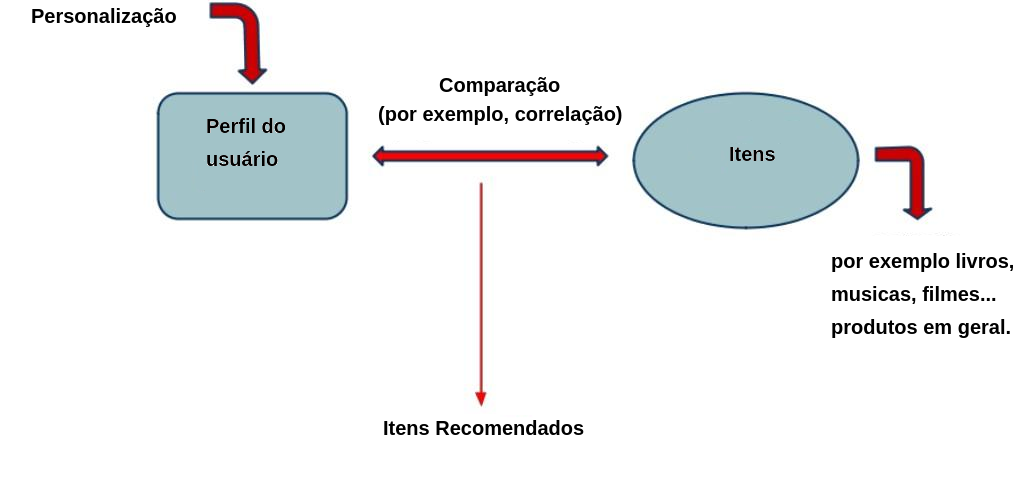
\includegraphics[scale=0.35]{figuras/referencial_teorico/sr_arquitetura.png}
    \caption[Arquitetura do sistema de recomendação em alto nível]{Arquitetura do sistema de recomendação em alto nível. Fonte: \cite{Stefanos:2008} de livre tradução do autor.}
    \label{fig:sr_arquitetura}
\end{figure}

Atualmente é possível comprar qualquer tipo de produto em lojas online, e isso gerou um evento conhecido como "Efeito Cauda Longa", como demonstrado na Figura \ref{fig:efeito_cauda}, na qual os produtos populares são poucos e podem ser encontrados com mais facilidade em lojas físicas ou em \textit{e-commerce’s}. Entretanto produtos não tão populares estão em maior quantidade e na grande maioria das vezes apenas é encontrado em sítios virtuas de de vendas \cite{pandey:2019}.

Não é por que o produto não é altamente popular que ele não vai ter uma boa qualidade, mas como esse tipo de produto é abundante, acaba que se torna um trabalho árduo pesquisar por algum, necessitando então de uma espécie de filtro. Nesse contexto que o sistema de recomendação pode ser empregado com sucesso.

\begin{figure}[H]
    \centering
    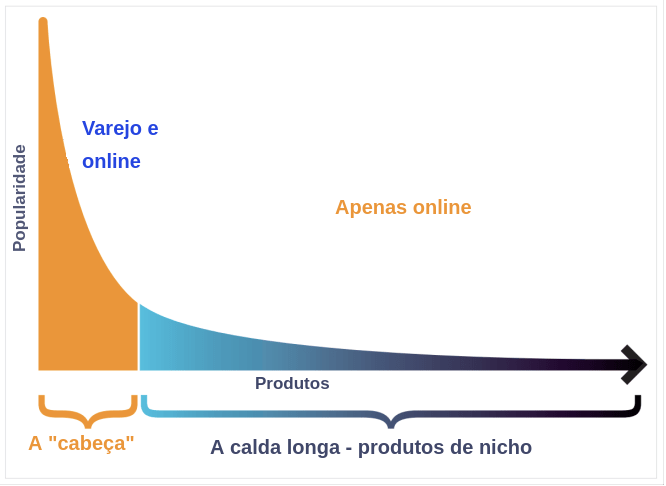
\includegraphics[scale=0.35]{figuras/referencial_teorico/efeito_cauda.png}
    \caption[Efeito Cauda Longa]{Efeito Cauda Longa. Fonte: \cite{pandey:2019} de livre tradução do autor.}
    \label{fig:efeito_cauda}
\end{figure}

\subsection{História do sistema de recomendação}

Segundo Sharma e Singh (\citeyear{Sharma:2016}), antes mesmo da existência de computadores os sistemas de recomendações já prevaleciam na sociedade. Civilizações antigas entre o período de 4000 a 1200 a.C, utilizavam do conceito de recomendações para fins de decisão no cultivo e até mesmo em âmbito religioso.

Durante o período de colonização, as recomendações ajudavam civilizações a escolherem territórios a se conquistar, analisando-se quesitos de fertilidade para agricultura ou de mão de obra. Reis, na era dos reinos, recebiam recomendações de seus ministros de quase todos os assuntos. Eles tinham o papel de manter seus pontos de vista a frente do rei, a fim de ajudá-lo a tomar a decisões mais facilmente. Famílias antigas arranjavam casamentos, pessoas decidiam na compra de produtos ou no caminho mais curto a se fazer de um local a outro. Em todos os casos se utilizavam recomendações para se realizar o que se desejava de maneira mais acertada ou coerente com os objetivos almejados \cite{Sharma:2016}.

Com a revolução industrial, o surgimento da era computacional foi possível, mudando completamente o mercado no mundo. Uma infinidade de produtos são postos à frente das pessoas e dessa forma gerando confusões no momento de decisão da compra, como por exemplo, saber se determinado produto realmente atende os requisitos de preferência de uma pessoa. Com a necessidade da existência de sistemas capazes de filtrar ou facilitar nos critérios de seleção, há, finalmente, o surgimento dos sistemas de recomendação \cite{Sharma:2016}.

Segundo Ekstrand, Riedl e Konstan (\citeyear{Ekstrand:2011:CFR:2185827.2185828}), foi reconhecido logo cedo na história da computação a capacidade de máquinas fornecerem recomendações. Grundy, um bibliotecário baseado em computador, é considerado de grande importância para o engajamento dos sistemas de recomendação. Ele era bastante primitivo, usava de entrevistas para obter informações com usuários a fim de agrupá-los em estereótipos e assim gerar recomendações  baseadas nas preferências de livros por estereótipo.

    Segundo Sharma e Singh (\citeyear{Sharma:2016}), os sistemas de recomendação se tornaram uma área de pesquisa em meados da década de 1970 na Universidade de Duke. Com o avanço nos estudos começaram a surgir abordagens como \textit{collaborative filtering} (filtragem colaborativa) no início dos anos 90 como soluções para sistemas online. O primeiro sistema de recomendação foi o \textit{Tempestry1}. Era um sistema manual com a abordagem de filtragem colaborativa, que possibilitava usuários procurarem por itens baseados em ações de outros usuários. Sistemas de recomendação com essa abordagem começaram a se tornar uma tendência e um tópico de interesse nas áreas de pesquisas como: interação humano computador, aprendizado de máquina e mineração de dados \cite{Ekstrand:2011:CFR:2185827.2185828}. 

Ao final dos anos 90, os sistemas de recomendação começaram a emergir e serem implementados comercialmente. Provavelmente, o maior exemplar dessa tecnologia foi o \textit{e-commerce} da Amazon.com que considerava o histórico de compras e ações do usuário para fazer recomendações de seus itens na plataforma desenvolvida. Logo em seguida, diversos outros negócios começaram a implantar esse tipo de tecnologia em seus sistemas online \cite{Ekstrand:2011:CFR:2185827.2185828}.

Com a quantidade e variedade crescente de informações no ambiente virtual da Internet e produtos para comercialização, os sistemas de recomendações se tornaram um meio valioso para lidar com esse tipo de problema de sobrecarga de informações, promovendo escolhas eficientes e rápidas para os seus usuários \cite{Ricci:2010}.

Segundo Ricci et al. (\citeyear{Ricci:2010}), o interesse por sistema de recomendação aumentou consideravelmente nos últimos anos e esse fato é visto por causa de  indicadores, como: \textit{sites} bem avaliados (Amazon.com, YouTube, Netflix, Yahoo, Tripadvisor, Last.fm, e IMDb) utilizarem de sistemas de recomendações e desempenharem um papel importante pro negócio, a existência de conferências e \textit{workshops} na área, o acolhimento desse tópico por instituições de ensino e a existência de pesquisas e desenvolvimento na área em revistas acadêmicas. Além disso, também ocorreu um grande marco, que seria a Netflix ter promovido de 2006 a 2009 o Netflix Prize, uma competição com o fim de premiar em 1 milhão de dólares a equipe que desenvolvesse o melhor algoritmo que melhorasse as recomendações de filmes para os usuários de sua plataforma de filmes e séries \cite{netflixprize:2009}.

\subsection{Funções de um sistema de recomendação}

Segundo Ricci et al. (\citeyear{Ricci:2010}), existem dois tipos de funções que um sistema de recomendações podem desempenhar, um referente ao provedor do serviço e o outro ao seu usuário (cliente). Um exemplo seria um sistema de recomendação para um \textit{e-commerce} imobiliário, em que a motivação primária do cliente ao entrar na plataforma é encontrar um imóvel adequado as suas necessidades, enquanto que para o provedor do serviço seria aumentar o número de imóveis comercializados.

Esses autores ainda descrevem algumas razões para provedores de serviço investirem em sistemas de recomendação, sendo estas razões relacionadas a seguir:

\textbf{Aumentar o número de itens vendidos}. Considerada a função mais importante para um sistema de recomendação comercial por gerar vendas adicionais comparadas as vendas advindas de um processo sem suporte de recomendações. Itens que são recomendados, em sua maioria, atendem as necessidades dos usuários, dessa forma cumprindo o objetivo do sistema de recomendação.

Sistemas de recomendação não-comerciais apresentam também muitas vezes objetivos semelhantes, mesmo que não haja custo para o usuário, como por exemplo, sítios virtuais de notícias que desejam aumentar o número de notícias lidas por usuários.

De forma geral, o principal objetivo de provedores de serviço em aplicar sistema de recomendação em seu negócio é aumentar a quantidade de usuários que aceitem as recomendações, fazendo comparação com a quantidade de usuários que navegam no sistema.

\textbf{Vender itens mais diversos}. Também considerada uma função muito importante para um sistema de recomendação, que possibilita para o usuário recomendações de itens que podem ser difíceis de serem encontrados “manualmente” (sem apoio de sistemas de recomendação). O provedor do serviço quer que todos os seus itens sejam vendidos, não somente os mais populares, dessa forma o sistema de recomendação apresenta itens que se adéquam as preferências de cada usuário, e assim apresentam itens, podendo ser populares ou não, para o usuário certo.

\textbf{Aumentar a satisfação do cliente}. Aumentar o satisfação do usuário em um sítio virtual ou aplicativo faz com que eles gostem do sistema, aumentando suas visitas e também a chance de aceitação de recomendações. Boas interfaces de interação com o usuário e recomendações interessantes e precisas são fatores relevantes na satisfação do cliente.

\textbf{Aumentar a fidelidade do usuário}. Tratar clientes antigos como valiosos é muito importante, pois em sistemas de recomendação, muitas vezes, é utilizada as interações dos usuários antigos como base para o seu modelo de recomendação pela classificação dos itens disponíveis. Assim, quanto mais interações os usuários fizerem, dependendo do modelo utilizado, seu modelo será refinado e poderá atender melhor as preferências dos clientes.

\textbf{Melhor entendimento do que o usuário quer}. Com as preferências dos usuários coletadas implícita ou explicitamente pelo sistema de recomendação, há a possibilidade de reutilização do conhecimento gerado por análises de dados, para outros objetivos, como melhorar o gerenciamento do estoque ou da produção do item. Um exemplo seria em plataformas de viagens recomendarem anúncios promocionais para determinado tipo de cliente baseado em sua preferência de lugares visitados.

O sistema de recomendação também desempenha várias funções referente ao usuário final. De acordo com Herlocker et al. (\citeyear{Herlocker:2004}), são elas:

\textbf{Anotação no contexto}. O sistema de recomendação vai enfatizar itens baseado em um contexto. Por exemplo, na interface de navegação de TV a cabo, há a listagem dos programas que vão passar e o sistema de recomendação vai apresentar o que vale a pena ou não assistir \cite{Ricci:2010}.

\textbf{Encontrar bons itens}. A principal tarefa de sistemas de recomendação é apresentar para o usuário uma lista específica e avaliada de itens, que são recomendações baseadas em previsões de quanto o usuário gostaria de tal item. Na maioria dos sistemas comerciais a probabilidade de recomendação gerada pelo modelo não é apresentada.

\textbf{Encontrar todos os itens bons}. A maioria dos sistemas de recomendação focam em recomendar somente alguns itens, mas existem casos que cabe apresentar todos os itens para um usuário. Um exemplo seria sistemas para recomendar casos para advogados que procuram precedentes, em que não se pode negligenciar um único caso. Para esse tipo de recomendação o número de falsos-negativos devem ser suficientemente baixos para ter uma excelente precisão no momento de recomendar os itens.

\textbf{Recomendar uma sequência}. Existem casos que são recomendados itens para o usuário mas em uma devida sequência que seja agradável ao mesmo. Como utilizado no sistema de recomendação do Yahoo \textit{Entertainment} (Entretenimento) na aba de musicas (launch.yahoo.com), que recomenda músicas para os usuários em uma devida sequência.

\textbf{Recomendar um agrupamento}. Sistemas de recomendação também podem sugerir um grupo de itens que combinados seriam melhor aceitos. Por exemplo, em ambientes de viagens normalmente são recomendados com os destinos seus pontos turísticos, restaurantes, hotéis entre outras recomendações combinadas \cite{Ricci:2010}.

\textbf{Apenas navegar}: A principal função de um recomendador é ajudar o usuário a tomar uma decisão baseado em suas preferências, mas nem sempre é assim, existem muitos usuários que utilizam o sistema sem um objetivo eminente e navegam simplesmente porque acham agradável. Nesses casos a interface, facilidade de uso e a natureza das informações importam muito mais do que a precisão do recomendador.

\textbf{Encontrar recomendações confiáveis}: É muito comum usuários não confiarem em recomendadores e é por isso que muitas vezes eles testam o recomendador, alterando seu perfil, por exemplo, para averiguar se o comportamento do recomendador está condizente com suas preferências. Por esse fato, muitos sistemas de recomendações oferecem esse tipo de funcionalidade que permitem usuários conseguirem testar o comportamento do recomendador.

\textbf{Melhorar o perfil}: Os usuários tendem a contribuir com avaliações nos sistemas com o intuito de melhorar seu perfil, e dessa forma melhorar a qualidade de recomendação recebida. É a função que a maioria dos sistemas de recomendação utiliza, e é primordial para a atribuição de recomendações personalizadas para os usuários.

\textbf{Expressar-se}: Alguns usuários não se importam com recomendações feitas para eles e sim em contribuir com suas avaliações, simplesmente pelo fato de se sentirem bem fazendo essa contribuição. Esse tipo de usuário normalmente avaliam anonimamente diversos itens e tem certa facilidade em fazer contribuições. Pode se dizer que é muito bom para o sistema fornecer mais dados e assim melhorar as recomendações para os outros usuários.

\textbf{Ajudar outros}: Muitas vezes, os usuários tem o objetivo de contribuir com avaliações de itens para que melhore nas recomendações de outros usuários. Essa função em sua maioria está vinculada a função de expressar-se, mas nem sempre elas andam juntas.

\textbf{Influenciar outros}: Considerado como um fator infeliz, alguns usuários têm a motivação de fazer avaliações de itens para influenciar declaradamente outros usuários na compra ou visualização dos itens. Um exemplo seria na situação em que usuários avaliam filmes antes mesmo deles serem lançados para fazer com que eles sejam recomendados,  e dessa forma influenciar as pessoas a assistirem.

\subsection{Abordagens de recomendações}

Como dito por Beliakov et al. (\citeyear{Beliakov:2011}), as justificativas usadas por sistemas de recomendação para recomendar itens para usuários, vão depender de fatores específicos  das aplicações e da forma de como os dados são coletados nos sistemas. Dessa maneira várias abordagens vêm sendo utilizadas para desenvolver sistemas de recomendações.

Nesta seção serão descritas as principais abordagens de recomendações, denominadas \textit{collaborative filtering} (filtragem colaborativa), \textit{content-based filtering} (filtragem baseada em conteúdo), \textit{knowledge-based recommender systems} (sistemas de recomendação baseados em conhecimento), \textit{hybrid recommender systems} (sistemas de recomendação híbridos) e \textit{critiquing-based recommender systems} (sistemas de recomendação baseados em críticas).

\subsubsection{Filtragem Colaborativa} 
\label{Collaborativefiltering}
A ideia principal dessa técnica, também conhecida como filtragem colaborativa, é que as pessoas que concordaram no passado tendem a concordar no futuro, ou seja, é possível analisar o histórico de cada indivíduo para predizer qual item ele gostará também, precisando apenas do histórico de preferência de um conjunto de usuários do sistema \cite{Nilashi:2013}.

Essa obtenção de dados de preferência se divide em duas categorias: classificação explícita e a classificação implícita. A primeira é uma taxa de 0 a 5 atribuída pelo próprio usuário em algum item. Esse procedimento é o \textit{feedback} mais direto para se obter o dado de preferência, mas que nem sempre é advindo de uma grande quantidade de dados. O segundo infere os gostos do sujeito indiretamente através de ações no \textit{site}, como: quantidade de visualizações, cliques, registro de compras passadas, ter escutado ou não a alguma música e entre outros \cite{luo:2018}.
	
Segundo Pazzani e Billsus (2007), conforme citado por Nilashi et al. (\citeyear{Nilashi:2013}), a filtragem colaborativa tem as seguintes características:

\begin{itemize}
    \item Criação de perfil do usuário através das classificações de usuários nos itens;
    \item Identificação de usuários com gostos parecidos que classificam itens de maneira semelhante para um usuário alvo usando alguma função de similaridade;
    \item Recomendar um ou vários itens para o usuário alvo que os usuários com gostos parecidos preferiram.

\end{itemize}

Essa filtragem para realizar a recomendação necessita relacionar duas coisas: item e usuário. Para realizar a comparação entre essas duas entidades têm se duas principais técnicas: abordagem de vizinhança e o modelo de fatores latentes. Na relação item a item, a modelagem do perfil do usuário para um item é feita com base nas classificações do usuário em outros itens semelhantes \cite{Koren:2015}.

Os métodos para detecção dessa semelhança se divide em dois tipos: o \textit{memory-based} (baseado em memória) e o \textit{model-based} (baseado em modelo). A seguir, serão detalhadas as duas categorias.

%\subsubsection{Baseado em memória}

\textbf{Baseado em memória}. Esse tipo tem como característica calcular as semelhanças entre vizinhos na memória do computador. Os dados de entrada são carregados um passo antes do cálculo de detecção e assim são utilizados para fornecer a recomendação \cite{Levinas2014AnAO}. Essa categoria se divide em dois métodos: \textit{User-based filtering} (filtragem baseada em usuários) e \textit{Item-based filtering} (filtragem baseado em itens).

%\subsubsection{User-based filtering}

\textbf{Filtragem baseada em usuários}. Usuários com gostos parecidos irão realizar classificações semelhantes nos mesmos itens, por isso, é certo dizer que as classificações obtidas de outros usuários com a mesma opinião do usuário alvo, pode ser usada para recomendar o usuário alvo \cite{Cimini:2019}.

%\subsubsection{Item-based filtering}

\textbf{Filtragem baseada em itens}. Itens parecidos foram classificados de forma bem semelhante pelo mesmo usuário. Para predizer as classificações para um item alvo B pelo usuário A, deve-se primeiro determinar um conjunto de itens que sejam semelhantes ao item alvo B, assim, as classificações desse conjunto serão usadas para prever se o usuário A irá gostar do item B \cite{Cimini:2019}.

Em outras palavras, ao invés de utilizar a semelhança de comportamentos das classificações dos usuários para recomendar, será usado a semelhança entre os padrões de classificação dos itens. Se um grupo de itens tendem a ter os mesmos usuários que gostam e que não gostam, então é certo dizer que eles são semelhantes \cite{Ekstrand:2011:CFR:2185827.2185828}.

O item-item ou \textit{item-based} (baseado em itens) foi criado com a ideia de corrigir a característica de má escalabilidade do \textit{user-based}, mas na prática acaba que não corrige totalmente. Ambos as abordagens necessitam achar a similaridade seja de usuário, seja de item, mas como na maioria dos sistemas há mais usuários do que itens, assim é mais econômico encontrar a similaridade pelo item do que pelo usuário \cite{Ekstrand:2011:CFR:2185827.2185828}.

\begin{figure}[H]
    \centering
    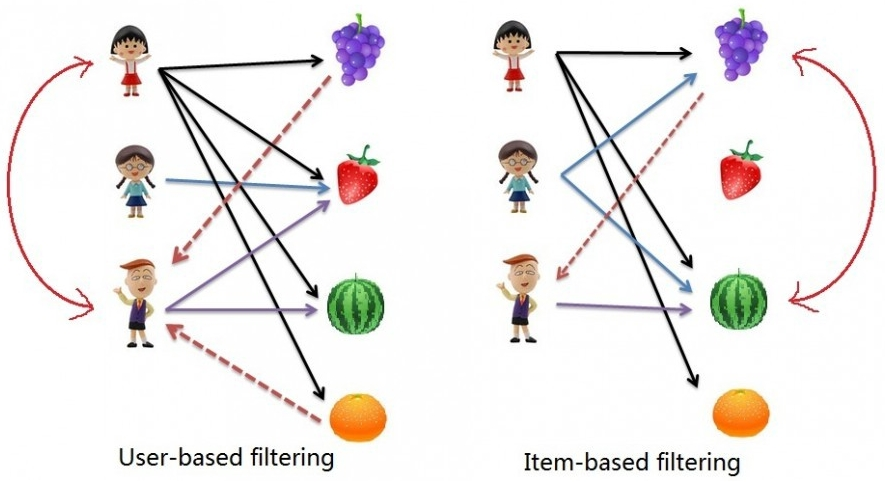
\includegraphics[scale=0.4]{figuras/referencial_teorico/user_based_item_based.jpg}
    \caption[User-based filtering e Item-based filtering]{User-based filtering e Item-based filtering. Fonte: \cite{Pinela:2017}}
    \label{fig:user_based_item_based}
\end{figure}

%\subsubsection{Baseado em modelo}

\textbf{Baseado em modelos}. Diferente do \textit{memory-based}, a categoria \textit{model-based} extrai informações de um conjunto de dados para criar um “modelo” que é utilizado calcular as recomendações. Geralmente é produzido um modelo \textit{offline} ao mesmo tempo que a recomendação acontece online. Foi graças ao Netflix \textit{Prize} que essa categoria recebeu um grande investimento nas comunidades de pesquisa \cite{Levinas2014AnAO}.

A escalabilidade aparece como o principal problema da abordagem, pois é necessário carregar uma grande quantidade de dados em memória no servidor para poder assim realizar a recomendação. Isso só piora quanto maior for a quantidade de usuários e de itens. Dessa forma ele demanda uma grande quantidade de recurso computacional e acaba pecando no desempenho do sistema. \cite{Grover:2017}.

Para finalizar, como descrito por Pinela (\citeyear{Pinela:2017}), os pontos positivos do \textit{collaborative filtering} são:

\begin{itemize}
    \item Não depende do contexto do sistema;
    
    \item Implementação simples;
    
    \item É mais preciso comparado a outras técnicas;
\end{itemize}

Mas também há alguns pontos negativos a se levar em consideração, como:

\begin{itemize}
    \item A porcentagem de usuários que avaliam itens em um sistema é relativamente baixa;
    
    \item Partida fria (\textit{cold start}): não irá ter muita informação de novos usuários para ser comparado com os outros usuários;
    
    \item Novo item: não haverá muitos dados sobre novos itens, dificultando a realização de uma classificação robusta.
\end{itemize}

\subsubsection{Filtragem baseada em conteúdo}
\label{Contentbasedfiltering}

Uma outra técnica muito usada em sistemas de recomendação é a também chamada filtragem baseada em conteúdo, na qual é analisado um conjunto de itens que são similares ao item já classificado pelo usuário anteriormente, e assim, é feito as recomendações para esse usuário. Essa similaridade se dá pela semelhança de características de um item classificado pelo próprio usuário com outro ainda não conhecido pelo usuário \cite{Grimaldi:2018}. 

Segundo Abbattista et al. (\citeyear{Abbattista:2002}), para analisar os desejos e gostos do usuário é necessário gerar um perfil deste, que é conhecido como \textit{user profile} (perfil do usuário). O perfil do usuário é um conjunto de várias informações que obtemos do usuário necessárias para recomendar um item para ele, extraídas a partir do momento em que ele entra no sistema.

Esse perfil é dado como uma lista de pares de atributos e valores, na qual cada atributo tem o seu respectivo valor, contendo determinada informação desse respectivo usuário. Como exemplo de atributos desse perfil, temos: idade, localidade, renda, gênero musical, gênero de filme, emprego, preferências e vários outros.

Esses atributos são divididos em três categorias:
\begin{itemize}
    \item \textbf{Explícito:} valores obtidos pelo próprio usuário;

    \item \textbf{Implícito:} dados obtidos através das ações do usuário;

    \item \textbf{Existente:} informações coletadas a partir de outro serviço já existente.
\end{itemize}

Com esse comportamento de encontrar a similaridade com as características do item, essa abordagem evita a falha de recomendar itens novos no sistema, descrita anteriormente, existente na abordagem de \textit{collaborative filtering}. \cite{Luk:2019}.

\begin{figure}[H]
    \centering
    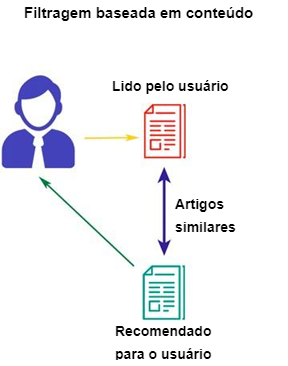
\includegraphics[scale=0.6]{figuras/referencial_teorico/content_based.png}
    \caption[Esquema do funcionamento do Content-based filtering]{Esquema do funcionamento do \textit{Content-based filtering}. Fonte: \cite{Jain:2019}}
    \label{fig:content_based}
\end{figure}

\subsubsection{\textit{Sistemas de recomendação baseados em conhecimento}}

Segundo Ricci et al. (\citeyear{Ricci:2010}), um sistema de recomendações baseado em um conhecimento específico de um domínio referente a como características dos itens satisfazem as necessidades e preferências dos usuários, ou de forma geral como um item é útil para um usuário, é considerado um sistema de recomendação baseado em conhecimento. O autor descreve que para esses sistemas, uma função de similaridade estima quanto um usuário corresponde a um item, ou seja, a similaridade corresponde a utilidade do item recomendado para um usuário.

Ainda segundo o autor a abordagem baseada em conhecimento tende a funcionar melhor que as outras no início de sua implementação mas caso não tenham recursos de aprendizado em sua implementação podem ser superados por outros métodos superficiais como o \textit{collaborative filtering}.

\subsubsection{Sistemas de recomendação híbridos}
\label{Hybrid}
Segundo Burke (\citeyear{Burke:2007}), sistemas de recomendações híbridos são combinações de duas ou mais abordagens descritas acima. Elas são feitas para melhorar a performance do recomendador e normalmente para sanar o problema de \textit{cold start}, como descrito no tópico da filtragem colaborativa anteriormente.

Existem diversas pesquisas na área que demonstram o sucesso do uso da abordagem híbrida para sistemas de recomendação. Essa abordagem tem a intenção de gerar um sistema de recomendação baseado no ponto forte de outros singulares. Ao usar mais de uma abordagem é possível uma compensar a falha de outra.

O autor descreve sete técnicas de hibridação utilizadas. São elas:

\begin{itemize}
    \item \textbf{\textit{Weighted}}: a pontuação de diferentes componentes de recomendação são combinados numericamente;
    
    \item \textbf{\textit{Switching}}: o sistema escolhe entre componentes de recomendação, seleciona um e o aplica;
    
    \item \textbf{\textit{Mixed}}: recomendações de diferentes recomendadores são apresentadas juntas;
    
    \item \textbf{\textit{Feature Combination}}: características derivadas de diferentes fontes de conhecimento são combinadas dadas a um único sistema de recomendação;
    
    \item \textbf{\textit{Feature Augmentation}}:  uma técnica de recomendação é usada para computar uma ou um conjunto de características, que será parte da entrada de outra técnica;
    
    \item \textbf{\textit{Cascade}}: os recomendadores recebem prioridade estrita, com os de menor prioridade quebrando os laços na pontuação dos mais altos;

    \item \textbf{\textit{Meta-level}}: uma técnica de recomendação é aplicada e gera alguma ordenação de um modelo que é a entrada de outro.

\end{itemize}

\subsubsection{\textit{Sistema de recomendação baseado em critica}}
\label{Critiquing-based}
Segundo Konstan e Riedl (2012), conforme citado por Chen e Pu (\citeyear{Chen:2012}), a tecnologia de recomendação, explorando similaridade nos usuários, pode ajudar usuários a encontrar itens ideais. Como descrito anteriormente, por exemplo, o \textit{collaborative filtering} tem a premissa de recomendar itens com alta classificação de usuários que avaliam os produtos para outros usuários semelhantes. Entretanto Chen e Pu (\citeyear{Chen:2012}) descreve que para domínios de itens de alto risco, como por exemplo uma propriedade ou um veículo, é provável que usuários façam pesquisas e realizem a compra de produtos pela primeira vez. Isso faz com que produtos sejam pouco avaliados, pois pessoas que não compram esse tipo de produto regularmente, não demonstraram sua opinião regularmente, e assim incapacitando sistemas que não vão conseguir estabelecer um perfil adequado para muitos de seus candidatos a recomendações.

Chen e Pu (\citeyear{Chen:2012}) descreve que para superar esse problema chamado de \textit{cold start}, como já descrito anteriormente, surgem os sistemas de recomendação baseados em crítica, que são amplamente reconhecidos por serem uma tecnologia de recomendação efetiva, assim como uma busca baseada em preferência efetiva que emprega um sistema de \textit{feedback} chamado \textit{critiquing} (criticar).

O autor afirma que nos sistemas baseados em crítica, inicialmente, as preferências do usuário não interferem na precisão da decisão, pois esse sistema se refere a um processo subsequente de críticas incrementais que ajudam os usuários a tomarem decisões mais informadas e precisas.

O sistema de recomendação baseado em crítica simula um vendedor artificial que inicialmente faz recomendações com base nas preferências atuais de um usuário e em seguida obtém \textit{feedback} do mesmo em forma de críticas, como por exemplo: “Gostaria de algo mais barato?”. É necessário que esse processo descrito seja em ciclos para que o usuário alcance seu produto ideal \cite{Chen:2012}. Segundo Pu (2000) e Faltings (2002), citado por Chen e Pu (\citeyear{Chen:2012}), um comprador normalmente tem muitas restrições e preferências que não são declaradas inicialmente, e ele só toma conhecimento quando as soluções propostas as violam.

Tipicamente, um sistema de recomendação baseado em crítica segue o modelo de interação sistema-usuário como apresentado na Figura \ref{fig:sistema_usuario} \cite{Chen:2012}.

\begin{figure}[H]
    \centering
    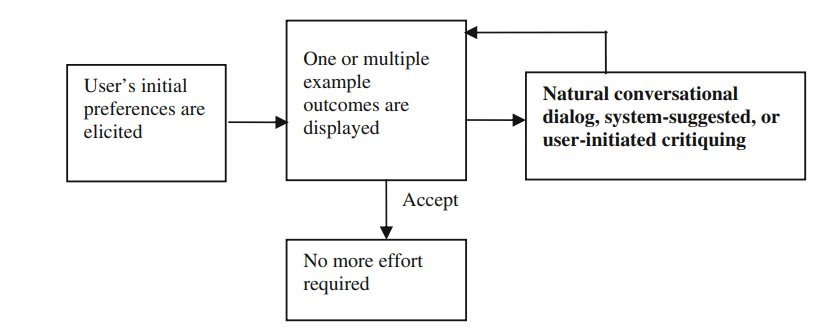
\includegraphics[scale=0.45]{figuras/referencial_teorico/sistema_usuario.png}
    \caption[Modelo de interação sistema-usuário]{Modelo de interação sistema-usuário. Fonte: \cite{Chen:2012}}
    \label{fig:sistema_usuario}
\end{figure}

Primeiramente o usuário atribui sua preferência, podendo ser um item de partida ou valores específicos sobre recursos dos itens. Em seguida o sistema recomenda um ou diversos itens para o usuário a partir de sua preferência inicial. Nesse momento um usuário seleciona um item podendo ser sua escolha final, mas normalmente ele escolhe um item quase desejável e dessa forma fará críticas sobre o item. O tipo de crítica que o usuário irá fazer vai depender do suporte a crítica do sistema. Uma vez que é feita a crítica o sistema irá atualizar suas recomendações, ou seja, refinando a preferência do usuário.

Os sistemas de recomendação baseados em crítica dão suporte a três tipos principais, São eles: \textit{natural conversational critiques}, \textit{system-suggested critiques} (críticas sugeridas pelo sistema), e \textit{user-initiated critiquing} (crítica iniciada pelo usuário) \cite{Chen:2012}.

\textbf{Crítica iniciada pelo usuário}. Segundo Pu and Chen (2005), como citado por Chen e Pu (\citeyear{Chen:2012}), a abordagem de crítica iniciada pelo usuário motiva usuários a fazer críticas estimulando-o com exemplos. Essa abordagem dá a liberdade para o usuário fazer a crítica para unidades ou qualquer combinação de recursos. O objetivo desse tipo de sistema é dar suporte ao usuário a executar livremente o \textit{trade-off} (troca). Isso pode ser definido como quando um usuário altera sua preferência referente ao valor de um atributo em particular. Esse processo melhora significativamente a precisão e confiança dos usuários.

Chen e Pu (\citeyear{Chen:2012}) descreve \textit{exemple-critiquing} (critica de exemplo) como um tipo de sistema que consiste em interface do usuário e uma ferramenta de busca. Inicialmente um usuário inicia sua busca especificando sua preferência por meio de uma área de consulta. Cada preferência é composta por valores de atributos e um peso atribuído a esse atributo, chamado de “importância”. Para a geração da recomendação é utilizado um modelo de preferência baseado em MAUT.

Segundo Keeney and Raiffa (1976) conforme citado por Chen e Pu (\citeyear{Chen:2012}), MAUT ou teoria da utilidade de atributos múltiplos, é uma teoria que leva em consideração preferências de valor conflitantes e produz uma pontuação para cada item. Chen and Pu (2007) , conforme citado por Kasamani (\citeyear{Kasamani:2017}), definem um modelo de preferência como o par \((V_1, ..., V_n, w_1, ..., w_n)\) onde \(V_1\) é o valor função e \(w_i\) o peso para cada atributo \(A_i\). A utilidade de cada item \((a_1, a_2, ..., a_n)\) pode ser computada utilizando a função de utilidade como mostrada na equação \eqref{funcaoUtilidade}.

\begin{equation}
    \label{funcaoUtilidade}
    U(<a_1,a_2,...,a_n>)=\sum_{i=1}^{n} w_i V_i(a_i)
\end{equation}

Após atribuída a primeira preferência do usuário o mecanismo de busca construído classifica-rá todos os itens com suas devidas pontuações, o que permitirá sua ordenação e assim o sistema retornará “k” principais itens. Segundo Faltings et al. (2004), como citado por Chen e Pu (\citeyear{Chen:2012}) normalmente são retornados entre 5 a 20 itens. Então o usuário aceita um item ou escolhe uma solução próxima e interage com o painel de \textit{trade-off} (troca), em que pode atribuir críticas. Em seguida, com um conjunto de críticas o sistema irá refinar o modelo de preferência do usuário juntamente com as importâncias (pesos) dos atributos. Por fim será recalculado e um novo conjunto de recomendações.

\section{\textit{Machine Learning}}
\label{machineLearning}
\subsection{O que é \textit{Machine Learning}?}

Segundo Mitchell (\citeyear{Mitchell:1997:ML:541177}) desde a invenção dos computadores nós seres humanos nos perguntamos se seria possível computadores aprenderem com a experiência automaticamente, e se seria possível entender e programá-los para esse fim. Ainda não se sabe como programar computadores para aprenderem tão bom quanto humanos, mas, nos dias atuais, existem algoritmos que são eficazes para certos tipos de tarefas de aprendizagem. 

Segundo Alpaydin (\citeyear{Alpaydin:2010:IML:1734076}) algoritmos são uma sequência de instruções em que se recebe umas entrada e se encontra uma saída. Por exemplo, um algoritmo pode ser feito para ordenar números. A entrada do algoritmo é uma lista de números desordenados e a saída uma lista de números ordenados.

Para algumas tarefas, entretanto, algoritmos não são capazes de estabelecer uma saída. Por exemplo, para identificar \textit{spams} em um conjunto de e-mails. Como entrada é passado um e-mail e como saída é desejado classificar entre “sim” ou “não” para spam. Não é possível identificar o que pode ser considerado um spam para todos os casos, pois isso é relativo de tempo em tempo e de individuo para individuo \cite{Alpaydin:2010:IML:1734076}.

O que é faltante em conhecimento, é compensado em dados. É possível, ainda referente ao exemplo dos e-mails, processar uma quantidade significativa de mensagens de exemplo, indicando ser um e-mail spam ou não, com o objetivo de “aprender” e conseguir classificar mensagens a partir disso. O que é desejável é encontrar um algoritmo para essa tarefa. Para algoritmos de ordenação, por exemplo, não é necessário “aprender” para ordenar, mas existem para várias situações, não um algoritmo, mas dados de exemplos \cite{Alpaydin:2010:IML:1734076}.


Segundo Witten et al. (\citeyear{Witten:2016:DMF:3086818}) o mundo atual está sobrecarregado de dados, e cada vez mais parece continuar e aumentar. Os computadores proporcionam armazenamento de dados para salvar coisas que antes provavelmente teria se jogado fora. Com avanço das tecnologias e dessa forma seu barateamento, existe um aumento no acesso de pessoas a computadores. A cada passo no mundo atual é mais um dado no banco de dados. A internet promove diversas informações, e a cada escolha que se faz, mais um registro é feito.	

Escondido nesses dados existem informações potencialmente úteis \cite{Witten:2016:DMF:3086818}. Banco de dados para os fins como exemplificados acima se tornam úteis somente quando analisados e transformados em informações que sejam possível fazer uso, como por exemplo para fazer predições. Nos exemplo dos e-mails, não é completamente randômico a forma em que as mensagens são escritas, há um padrão nessas mensagens, e analisando esse fator é possível fazer predições e classificar os e-mails \cite{Alpaydin:2010:IML:1734076}.

Segundo Witten et al. (\citeyear{Witten:2016:DMF:3086818}) \textit{machine learning} se trata de um campo do conhecimento em que são desenvolvidas técnicas para encontrar e descrever padrões estruturais em dados. Segundo o autor não a nada de novo em tentar encontrar padrões em dados. As pessoas vem procurando padrões em dados desde o início na humanidade. Os caçadores para encontrar sua caça, buscavam padrões na migração dos animais, agricultores buscavam padrões no crescimento das colheitas, políticos buscavam padrões na opinião dos eleitores e entre outras situações. 

Segundo Han, Kamber e Pei (\citeyear{Han:2011:DMC:1972541}), \textit{machine learning} investiga como computadores podem aprender ou melhorar sua performance baseado em dados. Ele diz ainda que a principal área de pesquisa refere-se a desenvolvimento de programas de computador que aprendem automaticamente a reconhecer padrões complexos e a tomar decisões inteligentes com base nos dados.

Segundo Alpaydin (\citeyear{Alpaydin:2010:IML:1734076}) a aplicação de métodos de \textit{machine learning} em grandes bases de dados é denominado de \textit{data mining}. Han, Kamber e Pei (\citeyear{Han:2011:DMC:1972541}) afirmam que \textit{data mining} é um assunto interdisciplinar e pode ser definido de várias maneiras diferentes. O autor considera "mineração de conhecimento a partir de dados" como um nome mais apropriado pois faz referência a mineração de conhecimento referente a grandes quantidades de dados.

Han, Kamber e Pei (\citeyear{Han:2011:DMC:1972541}) dizem ainda que muitas pessoas consideram \textit{data mining} como uma fase essencial do processo de descoberta de conhecimento. O processo é demonstrado na Figura \ref{fig:etapas_ml} que é uma sequência interativa de sete etapas existentes. Elas são descritas pelo autor como:

\begin{itemize}
    \item \textbf{\textit{Data cleaning} (Limpeza de Dados)}: Para remover dados inconsistentes;

    \item \textbf{\textit{Data integration} (Integração de Dados)}: Onde várias fontes de dados são combinadas;

    \item \textbf{\textit{Data selection} (Seleção de Dados)}: Onde os dados relevantes para a tarefa em análise são recuperados da base de dados;

    \item \textbf{\textit{Data transformation} (Transformação de Dados)}: Onde os dados são transformados e consolidados em formas apropriadas para mineração, executando operações de resumo ou agregação;

    \item \textbf{\textit{Data mining} (Mineração de Dados)}: Um processo essencial em que métodos inteligentes são aplicados para extrair padrões;

    \item \textbf{\textit{Pattern evaluation} (Avaliação de padrões)}: Identificar os padrões realmente interessantes que representam o conhecimento com base em medidas de interesse;

    \item \textbf{\textit{Knowledge presentation} (Apresentação de conhecimento)}: Onde as técnicas de visualização e representação de conhecimento são usadas para apresentar conhecimento extraído aos usuários.

\end{itemize}

\begin{figure}[H]
    \centering
    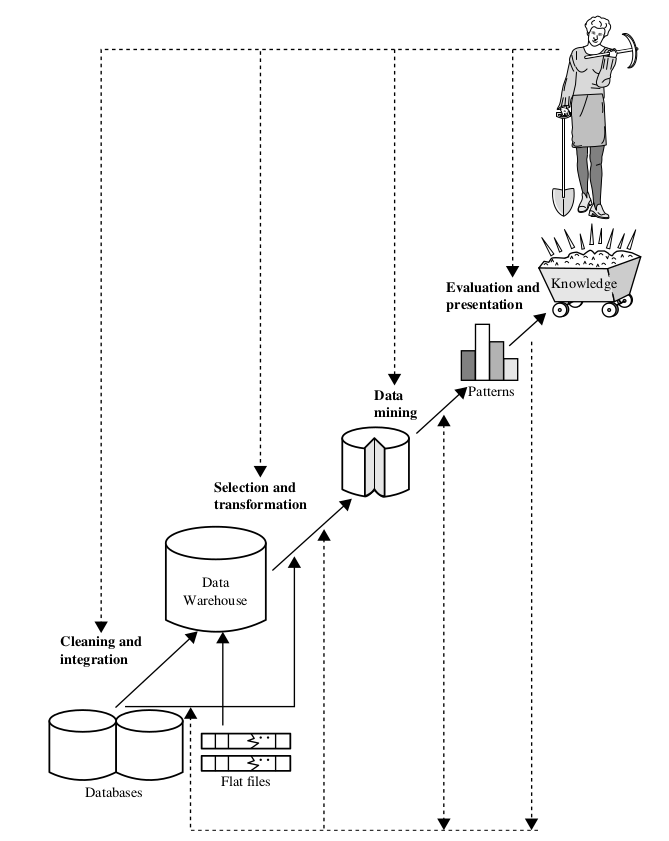
\includegraphics[scale=0.45]{figuras/referencial_teorico/etapas_ml.png}
    \caption[Etapas do processo de descoberta de conhecimento]{Etapas do \textit{machine learning}. Fonte: \cite{Han:2011:DMC:1972541}}
    \label{fig:etapas_ml}
\end{figure}

Dos passos um ao quatro, o autor considera como formas diferentes de pré-processamento de dados, que assim são propagados para mineração. Após os dados serem minerados eles são apresentados para o usuário ou postos em uma base de conhecimento. O dado apresentado pode ser ou não reaproveitado.

Dado que muitas outras áreas têm diferentes definições para \textit{data mining}, Han, Kamber e Pei (\citeyear{Han:2011:DMC:1972541}) definem-a como:

“Processo de descobrir padrões e conhecimentos interessantes a partir de grandes quantidades de dados. As fontes de dados podem incluir bancos de dados, \textit{data warehouses}, a \textit{Web}, outros repositórios de informações ou dados transmitidos dinamicamente para o sistema.” 

\subsection{Aprendizado indutivo}

Como dito anteriormente, o campo de \textit{machine learning} permitiu com que aplicações sejam capazes de aprender e melhorar seu desempenho por meio da observação. Segundo Batista (\citeyear{Batista}) existem diversas abordagens diferentes que podem ser utilizadas por uma aplicação como, por exemplo, o aprendizado por hábito, por instrução, por dedução, por analogia e por indução. O autor afirma que o aprendizado indutivo é um dos mais úteis pois possibilita novos conhecimentos a partir de exemplos ou casos previamente observados, mas também um dos mais desafiadores pois o conhecimento gerado ultrapassa os limites das premissas e ainda não há a garantia do conhecimento ser verdadeiro.

Monard e Baranauskas (\citeyear{Monard:2003}) definem a indução como uma forma de inferência lógica que possibilita a obtenção de conclusões genérica sobre um conjunto de exemplos. Ela é caracterizada por um raciocínio originário de uma generalização de um conceito específico, dessa forma, da parte para o todo. Para um conceito ser aprendido é feita uma inferência indutiva sobre os exemplos apresentados. Mesmo que as hipóteses geradas pela inferência poderem ou não preservar a verdade, é um dos principais métodos utilizados para derivar conhecimento novo e predizer eventos futuros.

Os autores definem que o aprendizado indutivo se divide em dois, supervisionado e não-supervisionado. No aprendizado supervisionado os dados apresentados ao algoritmo são exemplos postos a serem treinados e possuem o rótulo da classe associada conhecido. De maneira geral os exemplos são compostos de características e um rótulo da classe associada. O algoritmo de aprendizado tem como objetivo construir um classificador capaz de determinar a classe de exemplos ainda não rotulados. Para rótulos de classe com valores contínuos são definidos problemas denominados de “regressão”, para valores discretos  “classificação”.

Han, Kamber e Pei (\citeyear{Han:2011:DMC:1972541}) define aprendizado não-supervisionado essencialmente como sinônimo de \textit{cluster}. Ele não é supervisionado por seus exemplos de entrada não serem rotulados como classe. Normalmente é possível usar agrupamento para descobrir classes nos dados.

Para o presente trabalho será estudado e modelado uma solução em \textit{machine learning} para um problema de classificação supervisionada. A Figura \ref{fig:hierarquia_aprendizado} apresenta a hierarquia do aprendizado indutivo destacando a classificação.

\begin{figure}[H]
    \centering
    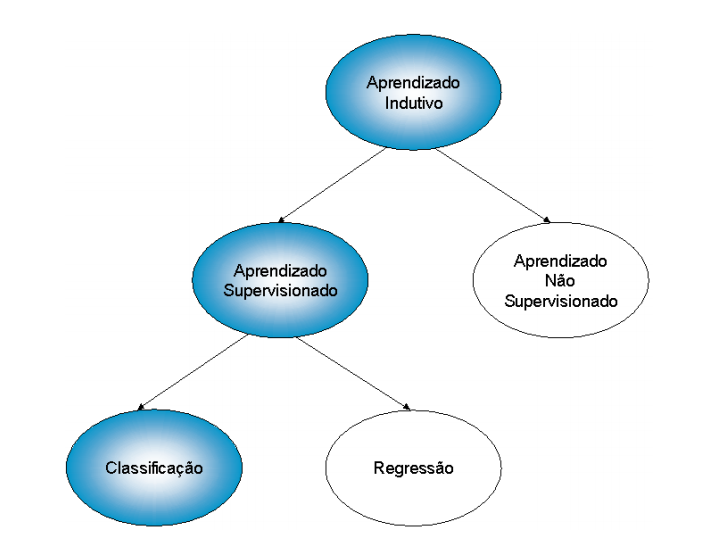
\includegraphics[scale=0.45]{figuras/referencial_teorico/hierarquia_aprendizado.png}
    \caption[Hierarquia do aprendizado indutivo]{Hierarquia do aprendizado indutivo. Fonte: (MONARD, 2003)}
    \label{fig:hierarquia_aprendizado}
\end{figure}

Para exemplificar, Monard e Baranauskas (\citeyear{Monard:2003}) apresentam o processo de classificação como na Figura \ref{fig:processo_classificacao}. Ele descreve que os dados de entrada do indutor são provenientes do conhecimento sobre um domínio. Após feita a indução o classificador é avaliado, podendo ou não ser repetido, dado que podem ser adicionado novos atributos ou exemplos, e ainda podem ser feitos ajustes nos parâmetros no processo de indução.

\begin{figure}[H]
    \centering
    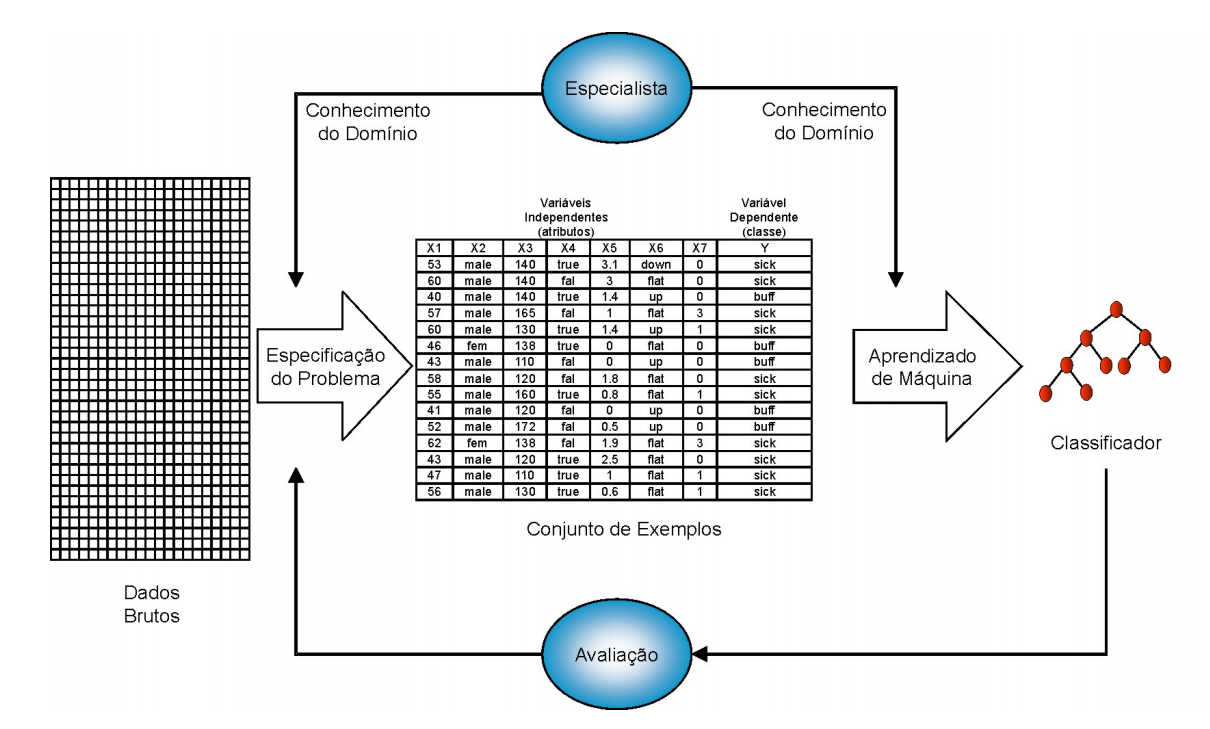
\includegraphics[scale=0.3]{figuras/referencial_teorico/processo_classificacao.png}
    \caption[Processo de classificação]{Processo de classificação. Fonte: \cite{Monard:2003}}
    \label{fig:processo_classificacao}
\end{figure}

\subsubsection{Questões gerais dos algoritmos de aprendizado supervisionado}
	
Segundo Kotsiantis (\citeyear{Kotsiantis}) o processo que descreve a aplicação de \textit{machine learning} supervisionada para um problema do mundo real é como apresentado no fluxograma representado na Figura \ref{fig:aplicacao_ml}.

\begin{figure}[H]
    \centering
    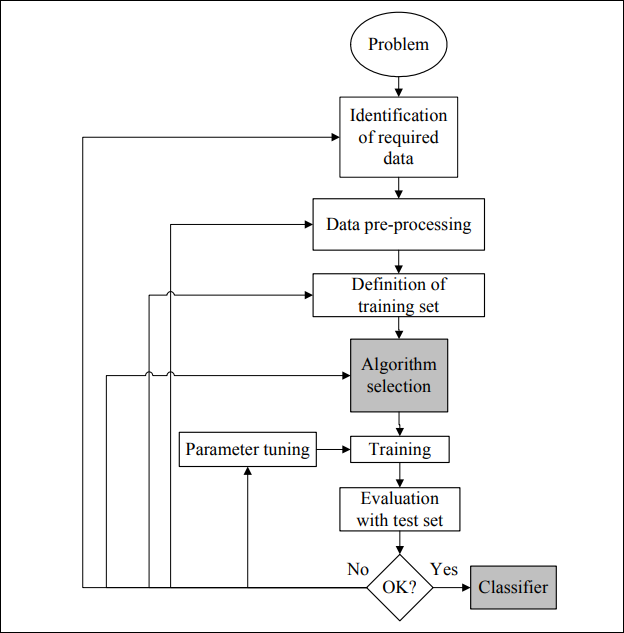
\includegraphics[scale=0.4]{figuras/referencial_teorico/aplicacao_ml.png}
    \caption[Aplicação de machine learning supervisionada no mundo real]{Aplicação de \textit{machine learning} supervisionada no mundo real. Fonte: \cite{Kotsiantis}}
    \label{fig:aplicacao_ml}
\end{figure}

O autor define o primeiro passo como a coleta de dados. Separar ou isolar quais são os campos mais informativos e relevantes para o problema. O segundo passo é o pré-processamento dos dados. Zhang et al. (2002), como citado pelo autor, considera um passo de muita importância, pois os dados podem ter ruídos e valores de recursos ausentes. Há diversas pesquisas referentes a detecção de dados faltantes e ruídos e como lidar com isso. Para lidar com esse tipo de problema muitas vezes é feita uma seleção de dados, que é considerada como um problema de otimização que tenta manter a qualidade da mineração minimizando o tamanho da amostra. Segundo Liu and Motoda (2001), conforme citado pelo autor Haverá uma redução nos dados, mas fará com que o algoritmo funcione efetivamente com vários grandes conjuntos de dados.

Em seguida vem a definição dos dados de treino. Segundo Yu e Liu (2004), conforme citado pelo autor Kotsiantis (\citeyear{Kotsiantis}), define como o processo de identificar e remover o máximo de campos ou características irrelevantes. Isso faz com que os algoritmos de \textit{data mining} operem mais rápidos e com mais eficácia, pois diminui a dimensionalidade dos dados. De acordo com o Markovitch e Rosenstein (2002), referidos por Kotsiantis (\citeyear{Kotsiantis}), muitas vezes há campos que dependem muito um do outro e isso é ruim, pois influenciam negativamente no modelo de \textit{machine learning}. Uma solução para isso é a aplicação da técnica de transformação ou construção de novos campos a partir de outros. Isso vai levar a classificadores mais concisos e precisos além de melhorar a sua compreensibilidade.

Logo após o passo de escolha do algoritmo de aprendizagem, que é de muita criticidade, os dados são treinados. Quando o teste preliminar é julgado satisfatório, um classificador é criado e está pronto para ser usado.

Para se avaliar um classificador é comumente usado a métrica de acurácia (porcentagem de previsões corretas dividido pelo número total de previsões). Segundo o autor existem pelo menos três técnicas para calcular a acurácia do classificador. Essas técnicas necessitam de uma base de dados de teste, normalmente obtidas pela divisão do conjunto de dados, que possibilitam no cálculo de acurácia.

Caso a taxa de erro encontrada seja insatisfatória, deve-se retornar para a etapa anterior do processo de classificação supervisionada. Fatores devem ser examinados com o propósito de melhorar o modelo. De acordo com Japkowicz e Stephen (2002), citado pelo Kotsiantis (\citeyear{Kotsiantis}), muitas vezes fatores como: características importantes não estão sendo usadas, base de teste está muito pequena, dimensionalidade do problema é muito alta, foi selecionado um algoritmo inadequado para o problema ou há a necessidade de ajustes em seus parâmetros e ainda o conjunto de dados está desequilibrado. Uma forma comum de se comparar algoritmos para encontrar a melhor escolha, é por meio de comparações estáticas da acurácia para um determinado conjunto de dados de teste.

Para os chamados “sistemas inteligentes”, a classificação supervisionada é tarefa mais realizada. Dessa forma foram desenvolvidas várias técnicas baseadas em inteligência artificial, Perceptron e Estatísticas.
	
\subsubsection{Método \textit{Ensemble}}
\label{ensemble}
Segundo Sirikulviriya e Sinthupinyo (\citeyear{SirikulviriyaIntegrationOR}) existe uma técnica muito popular de \textit{machine learning}, de grande interesse nas comunidades de \textit{data mining}, que é chamada de método \textit{ensemble} (conjunto). Ele afirma que é amplamente aceito que a precisão do conjunto de vários classificadores fracos (classificadores com baixa capacidade preditiva) é geralmente melhor que um único classificador, dada a mesma quantidade de dados de treino. Algoritmos eficazes diversos foram inventados para tal função nos últimos 15 anos, como por exemplo: \textit{Bagging} (Ensacamento), \textit{Boosting} (Aumento), \textit{Arching} (Arquear) e \textit{Random Forest} (Floresta Aleatória).

\textbf{\textit{Random Forest}}. É um classificador \textit{ensemble} proposto por Breiman (\citeyear{Breiman:2001:RF:570181.570182}). De forma geral, a forma utilizada para criação deste classificador é a construção de várias árvores de decisão, em que cada uma utiliza um subconjunto de atributos selecionados aleatoriamente.

Segundo Mitchell (\citeyear{Mitchell:1997:ML:541177}), conforme citado por Amal (\citeyear{Amal}) árvores de decisão categorizam as instâncias ou exemplos, como um arranjo de uma árvore, definindo-as da raiz a um nó de folha específico. Todo nó na árvore representa um teste referente a algum atributo da instância, enquanto cada ramificação descendente do nó representará um valor de um atributo. O autor sugere um exemplo como mostrado na Figura \ref{fig:arvore_decisao}. Ele descreve que a árvore de decisão foi construída com base no atributo “perspectiva”, em que existem três valores: nublado, ensolarado e chuvoso. Há também valores com subárvores como chuvoso e ensolarado. Ao final será classificado entre brincar e não brincar nesse dia de acordo com a distribuição de exemplos de maior quantidade na folha, que inicialmente nove eram para brincar e cinco para não brincar. Como dito anteriormente e agora reforçado por Mitchell (\citeyear{Mitchell:1997:ML:541177}), a classificação de exemplos em um conjunto distinto de prováveis agrupamentos é denominado como problema de classificação.

\begin{figure}[H]
    \centering
    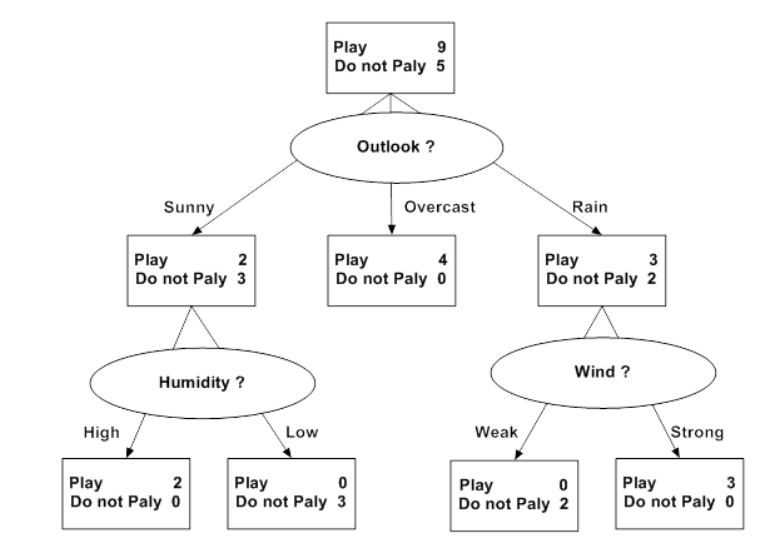
\includegraphics[scale=0.4]{figuras/referencial_teorico/arvore_decisao.png}
    \caption[Exemplo de uma árvore de decisão]{Exemplo de uma árvore de decisão. Fonte: \cite{Amal}}
    \label{fig:arvore_decisao}
\end{figure}

Para o modelo de árvore é inicialmente alcançado a categorização em grupos de observações. Após isso segue com a pontuação dos grupos específicos gerados. É possível definir modelo de árvore como um processo de procedimento recursivo em que uma quantidade de unidades estáticas, em um conjunto, são postas em grupos. O agrupamento das unidades existentes dependem de dadas regras de divisão que são progressivas. O principal objetivo da regra de divisão é a maximização da homogeneidade ou a medida da pureza da variável de resposta em seu grupo, conforme elas vão sendo obtidas. A regra de divisão executa uma forma de dividir as observações, em que cada característica a ser dividida e a regra de divisão definida são essenciais no procedimento de divisão do processo. O principal resultado de uma árvore de decisão é a partição final das observações \cite{Amal}. 

Segundo Thomas (\citeyear{Thomas:2017}) a árvore de decisão é uma técnica de modelagem de \textit{machine learning} não paramétrica amplamente utilizada. Métodos não paramétricos são quando não há suposições subjacentes sobre a distribuição dos erros ou dos dados, ou seja o modelo é construído baseado na observação dos dados.

Segundo Breiman (\citeyear{Breiman:2001:RF:570181.570182}), citado por Drummond (\citeyear{Drummond:2017}), o \textit{random forest} cria, a partir de um treinamento único, diversas árvores de decisão para fora do subconjunto de dados. Esse treinamento é feito utilizando algoritmo de \textit{bagging}, um método utilizado para melhorar a classificação ou regressão de modelos a partir da estabilidade e precisão da classificação. O \textit{random forest} faz sua predição conforme sua decisão por meio da contagem de votos dos componentes preditores de cada classe. Dessa forma é selecionada uma classe vencedora referente do número de votos acumulados para cada classe.

\begin{figure}[H]
    \centering
    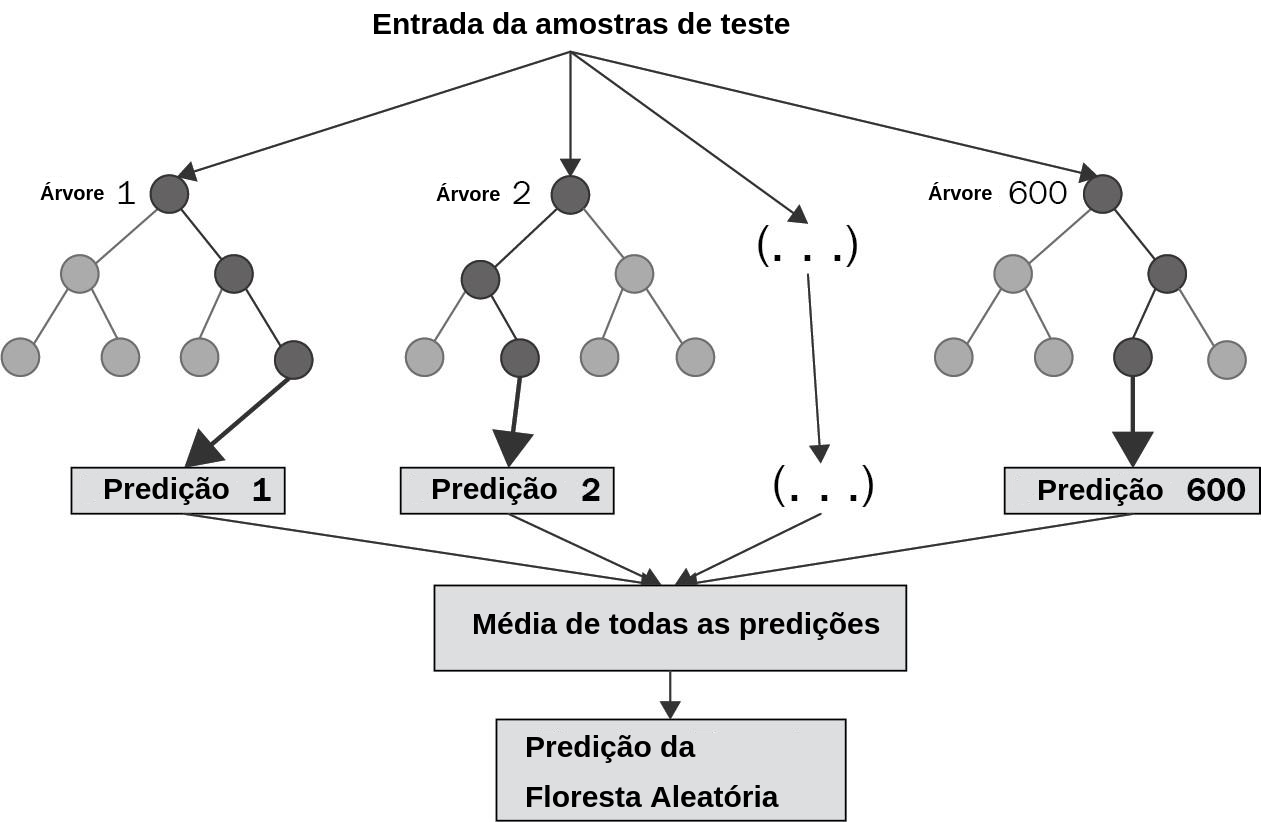
\includegraphics[scale=0.3]{figuras/referencial_teorico/random_forest.png}
    \caption[Estrutura do random forest]{Estrutura do random forest. Fonte: \cite{Chakure:2019}}
    \label{fig:random_forest}
\end{figure}



\textbf{\textit{Boosting}}. Segundo Mayr, Binder, Gefeller e Schmid (2014) conforme citado por Vecmanis (\citeyear{Vecmanis:2019}), \textit{boosting} é também um classificador ensemble baseado em algoritmos semelhante ao \textit{random forest}. Ele cria um modelo preditivo mais preciso por meio de uma otimização passo a passo, que envolve uma sequência de várias iterações analíticas.  De forma geral qualquer classificador fraco pode ser potencialmente melhorado (\textit{boosted}) para se tornar também um classificador forte.

Segundo o Hoare (\citeyear{Hoare:2019}), o \textit{machine learning boosting} começa treinando um modelo inicial, com por exemplo utilizando uma árvore de decisão. Em seguida, é construído um segundo modelo que se concentra em prever com melhor precisão os casos em que o primeiro apresentou baixa precisão. Dessa forma é esperado que a combinação desses dois modelos seja melhor que apenas um. A cada modelo sucessivo, tenta-se corrigir as deficiências da combinação do conjunto de árvores de decisão anteriores.

\textit{Gradient boosting} (Aumento de gradiente) é um algoritmo de \textit{machine learning boosting}. A ideia principal para encontrar um melhor modelo posterior, com a combinação de outros modelos, é na minimização do erro de previsão total. Ele funciona estabelecendo saídas (\textit{targets}) para o modelo posterior a fim de minimizar o erro. Para calcular essa saída a ser estabelecida vai depender de quanto a alteração da previsão desse caso (linha do \textit{dataset} de treino) afeta o erro total de previsão. Se uma pequena alteração na previsão de um caso causar uma grande queda no erro, o próximo resultado desejado do caso será um valor alto. As previsões do novo modelo que estão próximas de seus objetivos reduzirão o erro. Se uma pequena alteração na previsão de um caso não causar alteração no erro, o próximo resultado desejado do caso será zero, pois alterar essa previsão não diminuirá o erro. O \textit{gradient boosting} (gradiente descendente) é assim denominado porque os resultados de destino para cada caso são definidos com base no gradiente descendente do erro em relação à previsão \cite{Hoare:2019}.

\begin{figure}[H]
    \centering
    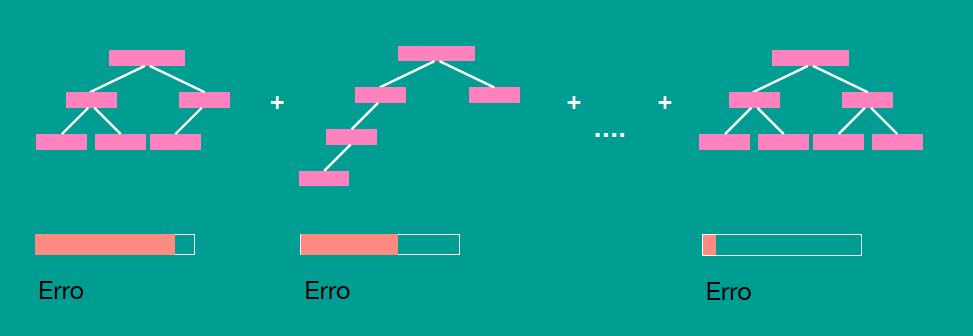
\includegraphics[scale=0.4]{figuras/referencial_teorico/gradient_boosting.png}
    \caption[Gradient Boosting]{Gradient Boosting. Fonte: \cite{Chepenko:2019}}
    \label{fig:gradient_boosting}
\end{figure}
 
Para deixar mais claro a ideia do conceito de \textit{gradient descent} (gradiente descendente), Ben (\citeyear{Ben:2017}) apresenta o seguinte exemplo: uma função de perda (\textit{loss function}), L, capaz de calcular o erro de previsão total, se apresenta como na equação \eqref{lossFunction}.
 
 \begin{equation}\label{lossFunction}L(x_1, x_2)=\frac{1}{2}(x_1-15)^2+\frac{1}{2}(x_2-25)^2\end{equation}

O objetivo é encontrar o par \((x_1, x_2)\) que minimiza a função \(L\). Ela pode ser interpretada como calculando o erro ao quadrado para dois pontos de dados, 15 e 25, com dois valores de previsão, \(x_1\) e \(x_2\). Para essa função demonstrada acima é possível minimizá-la diretamente, mas o \textit{gradient descent} (gradiente descendente) nos permitirá minimizar funções de perda mais complicadas que não são possíveis de minimizar diretamente.
